
\section{The big picture}
Basic though it may seem, the combined model of algebra is to sequence the 
invention of new numbers, learn to compute with them, find relatinships 
between solutions, and use that to reinvent numbers.
\begin{center}
    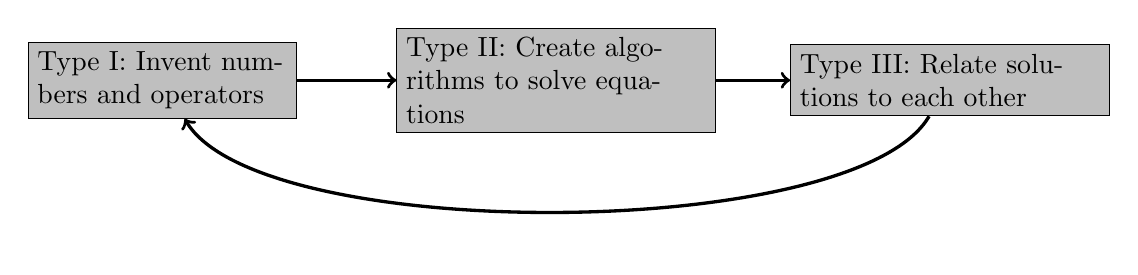
\begin{tikzpicture}
        \node[text width=1.25in, draw,fill=black!25] (a) at (0,0) {Type I: Invent numbers and operators};
        \node[text width=1.5in, draw,fill=black!25] (b) at (5,0) {Type II: Create algorithms to solve equations};
        \node[text width=1.5in, draw,fill=black!25] (c) at (10,0) {Type III: Relate solutions to each other};
        % \draw[very thick,->] (-4,0) -- (a);
        \draw[very thick,->] (a) -- (b);
        \draw[very thick,->] (b) -- (c);
        \draw[very thick,->] (c) edge[looseness=0.5,out=-120,in=-60] (a);
    \end{tikzpicture}
\end{center}


Yet to get started we better understand what it means to substitute 
for variables that can be $+$ signs and $=$ signs.
\begin{itemize}
    \item[$\Box$] What is an equation? (A pair of formulas form the same unambiguous context-free grammar.)
    \begin{itemize}
        \item[$\Box$] What is a context-free grammar? (A model for expressing complex induction.)

        \item[$\Box$] What is a variable? (An element of the variable alphabet.)

        \item[$\Box$] What makes an operator-variable? (A production rule in a context-free grammar.)

        \item[$\Box$] What is a formula? (A parse-tree of a context-free grammar.)
        
        \item[$\Box$] What is equality? (A variable with the Leibniz law as elimination.)

    \end{itemize}

    \item[$\Box$] What is an algebra? (A collection of types and operators matched to the 
    production rules of a context-free grammar.)
    \begin{itemize}
        \item[$\Box$] What substitutes for an operator in a formula? 
        (A $\lambda$ which can be typed to match the production rules of the grammar.)

        \item[$\Box$] What substitutes for a variable in a formula?
        (Terms of of the types matched to the grammar.)
        
        \item[$\Box$] What substitutes for equality in a formula? 
        (A congruence on the algebra.)
    \end{itemize} 
    
\end{itemize}
